\documentclass[tikz]{standalone}

\usepackage{pgfplots}

\usepackage[utf8]{inputenc}
\usepackage[T1]{fontenc}
\usepackage{times}

\begin{document}

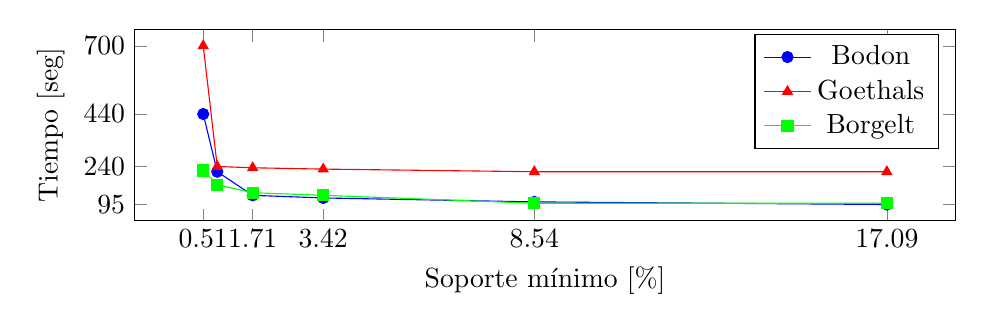
\begin{tikzpicture}
	\begin{axis}[width=12cm,
							height=4cm,
							xtick={17.09,8.54,3.42,1.71,0.51},
							ytick={95,240,440,700},
							%title={Nuestros datos},
							xlabel={Soporte m\'inimo [\%]},
							ylabel={Tiempo [seg]},
							xticklabel style={/pgf/number format/.cd,fixed,precision=3}
							]
		\addplot[color=blue,mark=*] coordinates {(17.09,95) (8.54,105) (3.42,120) (1.71,130) (0.85,220) (0.51,440)};
		\addlegendentry{Bodon}
		\addplot[color=red,mark=triangle*] coordinates {(17.09,220) (8.54,220) (3.42,230) (1.71,235) (0.85,240) (0.51,700)};
		\addlegendentry{Goethals}
		\addplot[color=green,mark=square*] coordinates {(17.09,100) (8.54,100) (3.42,130) (1.71,140) (0.85,170) (0.51,225)};
		\addlegendentry{Borgelt}
	\end{axis}
\end{tikzpicture}

\end{document}
